\documentclass{article}
\usepackage[utf8]{inputenc}
\usepackage{amsmath, amsthm, amsfonts,amssymb}
\usepackage[spanish]{babel}
\usepackage{multicol}
\usepackage{listings}
\lstset{basicstyle=\footnotesize\ttfamily,breaklines=true}
\usepackage{alltt}
\usepackage{graphicx}
\usepackage{subfigure}
\usepackage{subfig}
\usepackage{float}
\usepackage{url}
\usepackage{enumerate}
\usepackage{framed}
\usepackage{color}
\usepackage{cancel}
\usepackage{wrapfig}\definecolor{shadecolor}{RGB}{250,250,250}
\usepackage{framed}
\usepackage{epstopdf}
\setlength\parindent{0pt}
\usepackage{listings}
\usepackage{color} %red, green, blue, yellow, cyan, magenta, black, white
% Operadores matemáticos y simbolos
\DeclareMathOperator{\dive}{div}
\DeclareMathOperator{\trace}{trace}
\DeclareMathOperator{\tr}{tr}
\DeclareMathOperator{\symm}{symm}
\DeclareMathOperator{\sk}{skew}
\DeclareMathOperator{\grad}{grad}
\DeclareMathOperator{\Grad}{Grad}
\DeclareMathOperator{\curl}{curl}
\DeclareMathOperator{\Curl}{Curl}
\def\R{\mbox{\(\mathbb{R}\)}}
\def\E{\mbox{\(\mathbb{E}\)}}
\def\P{\mbox{\(\mathbb{P}\)}}
\def\I{\mbox{\(\mathbb{I}\)}}
\def\L{\mbox{\(\mathbb{L}\)}}
\def\dx{\mbox{\(\,\mathrm{d}x\)}}
\usepackage{geometry}
\geometry{left=2.5cm, right=2.5cm, top=2cm, bottom=3cm}
\title{Tarea 2\\Cálculo Científico}
\author{Luis Felipe Silva De Vidts}
\begin{document}
\begin{figure}
\begin{minipage}{2.5cm}

\includegraphics[width=0.8\textwidth]{./figures/LogoUC-BN}
\end{minipage}
\begin{minipage}{14.5cm}
\vspace{4mm}
{\sc PONTIFICIA UNIVERSIDAD CAT\'OLICA DE CHILE}\\
Departamento de Matemáticas y Programa de Ingeniería Matemática y Computacional \\
{\bf IMT2111 Algebra Lineal Numérica}\\
\vspace{0mm}
\hrulefill
\end{minipage}
\end{figure}
\phantom{""}
\vspace{-5mm}
\normalsize
\begin{center}
\Huge Tarea 1\\
\normalsize Luis Felipe Silva De Vidts
\end{center}
\section*{Pregunta 2}
Considerando un computador cuyo sistema numérico es el conjunto $\mathbb{F}(10,5,-9999,9999)$
\begin{enumerate}[a)]
\item El epsilon de la máquina será:\\
$$\beta^{1-t} = 10^{1-5} = 10^{-4} $$
\item El número positivo más pequeño representable en $\mathbb{F}$ será:\\
En caso de ser un sistema normalizado, $\beta^{L-1}$ que en este caso es equivalente a 
$$10^{-10000}$$
mientras que para el caso desnormalizado será $\beta^{L-t}$ que en este caso será:
$$10^{-10004}$$
\end{enumerate}
\section*{Pregunta 3}
Al evaluar las expresiones en Python 3.5, usando infinito como \texttt{numpy.inf} y nan como \texttt{numpy.nan}	obtuve:
\begin{enumerate}[a)]
\item $1^{\infty}=1$
\item $2^{\infty}= \infty$
\item $e^{\infty}=\infty$ y $e^{-\infty}=0$
\item $sign(nan) = nan$ y $sign(-nan)= nan$\\ en ambos casos acompañados por un error de haber ingresado mal un dato en la función $sign(x)$
\item $nan^{0}=1$
\item $\infty^{0}=1$
\item $1^{nan}=1$
\item $\log(\infty)= \infty$, $\log(-\infty)= nan$ y $\log(0)= -\infty$\\ donde en los dos últimos casos el programa lanzo un error, de ingresar mal un dato y de división por 0 respectivamente.
\end{enumerate}
Considero que se obtuvieron los valores esperados, ya que aun que no es del todo correcto en algunos casos, se sigue una misma norma que permite seguir operando a pesar de que se tenga algun error.
\section*{Pregunta 4}
Al implementar la rutina que calcula $\sqrt{x}$ al tener una aritmética de punto flotante restringida no siempre se cumplirá que $\sqrt{x^{2}}=|x|$ ya que si se toma un $x$ muy grande o muy pequeño y se eleva al cuadrado en caso de ser muy pequeño se podría obtener un underflow y que en vez de obtener el modulo de $x$ obtendríamos $0$, o por otra parte si $x$ es muy grande $x^{2}$ podría retornar un overflow lo que el computador considerará como infinito o dirá que hay un error.\\
Mientras que si se aplica primero la raíz y luego la potenciación no se provoca este problema porque para números muy grandes sacar raíz retorna un número más pequeño que el ingresado y para un número muy pequeño entrega un número mayor, por lo que mantiene los números dentro del rango al que se puede entregar números de punto flotante donde el error esta acotado.\\
\section*{Pregunta 6}
Se pedía calcular el valor de $e^{x}$ mediante su serie de Taylor;
\begin{enumerate}[a)]
\item Utilizando aritmética de punto flotante de 3 dígitos (asumí mantisa de largo 3) obtuve como resultado $e^{0.1}\approx 1.105$
\item Obtuve un error absoluto de $1.7*10^{-4}$ (ocupando los números del computador normales el error es de $8.47*10^{-8}$) y un error relativo de$1.54*10^{-4}$
\item Ahora para $x=2.0$ se obtiene un error absoluto de $0.39$ y un error relativo de $0.0526$, el aumento del error se debe a que el modelo teórico toma como centro al $0$, si ocupáramos la seria completa no tendríamos ese error pero al truncarla se generan errores y cada vez mayores a medida que uno se aleja del $0$.
\item Para este caso con la primera aproximación obtuve:
$$e^{-5}\approx \sum_{k=0}^{9}\frac{(-5)^{k}}{k!}= -1.827 $$
mientras que para la segunda obtuve como resultado
$$e^{-5}\approx \frac{1}{\sum_{k=0}^{9}\frac{5^{k}}{k!}}= 0.006959$$
\item Considero que la segunda forma es más exacta dado que la aproximación es más certera en ese caso para ese valor de $k$, además como la primera es una suma oscilante, esta requiere más iteraciones para disminuir el error, mientras que de la otra forma solo se suman números positivos y se evita esa oscilación junto con la pérdida de dígitos significativos asociada a la aritmética de punto flotante.
\end{enumerate}
\section*{Pregunta 9}
Se pide ajustar las expresiones para evitar la pérdida de dígitos significativos\\

d)  $\sqrt{1+x}-1$ con $x\approx 0$\\
Para este caso usamos el teorema del binomio de Newton para escribir de otra forma la raíz
$$\sqrt{1+x} = (1+x)^{\frac{1}{2}}= 1+\frac{1}{2}*x + O(x^{2})$$
como $x\approx 0$ nos podemos quedar con la igualdad 
$$\sqrt{1+x}=1+\frac{x}{2}$$
Luego al reemplazar nos quedará 
$$1+\frac{x}{2}-1=\frac{x}{2}$$
Entonces 
$$\sqrt{1+x}-1 = \frac{x}{2}$$ 
Cuando $x\approx 0$.\\

f) $\frac{1-\cos(x)}{\sin(x)}$, para $x\approx 0$\\

Para este caso tomaremos las series de Taylor del coseno y seno.
$$\cos(x) = 1- \frac{x^{2}}{2}+O(x^{4}) $$
$$\sin(x) = x -O(x^{3})$$
podemos despreciar los elementos de mayor orden ya que $x\approx 0$ luego al reemplazar en la exprsión original tenemos
$$\frac{1-\cos(x)}{\sin(x)}=\frac{1-1+\frac{x^{2}}{2}}{x}=\frac{x}{2}$$
\section*{Pregunta 15}
Al usar la aproximación de Stirling
$$n! \approx \sqrt{2\pi n} * \left(\frac{n}{e}\right)^{n}$$
Para obtener el factorial de un número, al probar para $n \in \{1,2,3,\dots,12\}$ obtuve los siguientes errores absolutos y relativos.\\

\begin{figure}[h!]
\centering
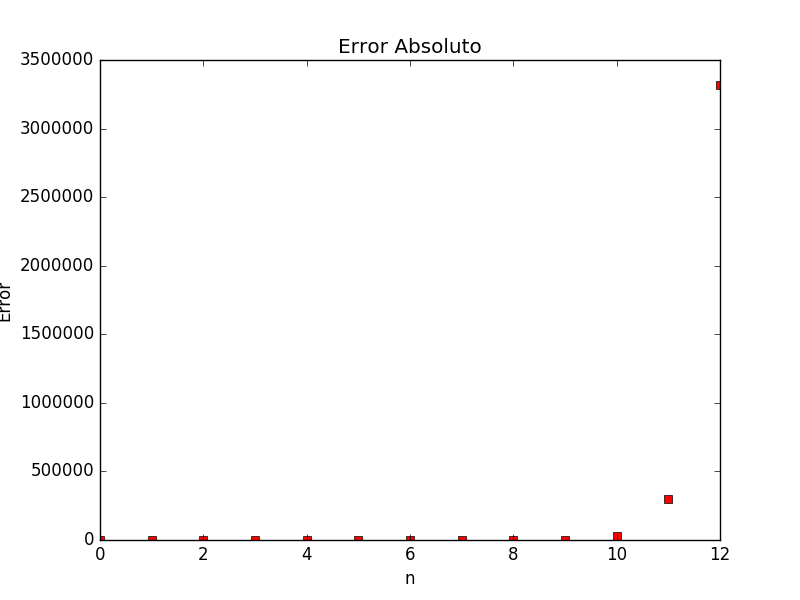
\includegraphics[scale=0.5]{Error_absoluto.png}
\caption{Error absoluto}
\end{figure}
Notamos que a medida que aumenta el valor de $n$ aumenta de forma exponencial el valor del error.\\
\\

\begin{figure}[h!]
\centering
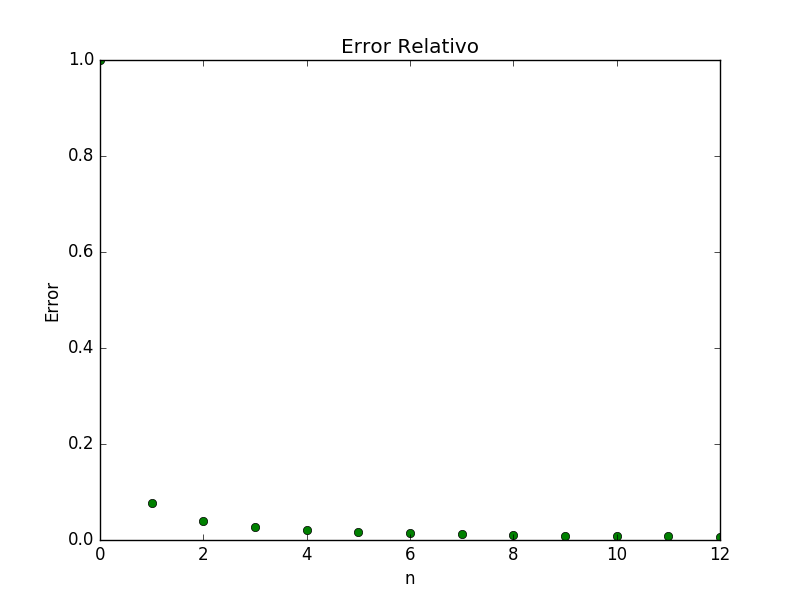
\includegraphics[scale=0.5]{Error_relativo.png}
\caption{Error relativo}
\end{figure}
Por otro lado el error relativo es cada vez menor, cuando $n =12$ es casi cero.\\

Dado lo anterior considero que la aproximación de Stirling para el factorial es una buena aproximación cuando $n\geq 10$, ya que a pesar de tener un gran error absoluto, como la escala a la que se encuentra es un error aceptable.

\section*{Pregunta 17}
Se pide explicar porque ocurre el fenómeno que se aprecia en el siguiente gráfico
\begin{figure}[h!]
\begin{minipage}{8 cm}
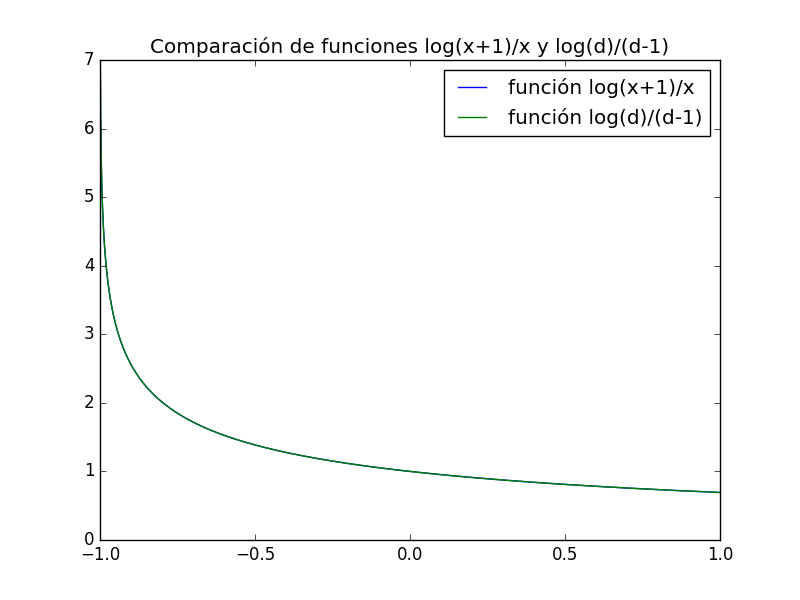
\includegraphics[scale=0.4]{Comparacion_funciones_2.png}
\caption{Gráfico para $x\in [-1,1]$}
\end{minipage}
\begin{minipage}{8 cm}
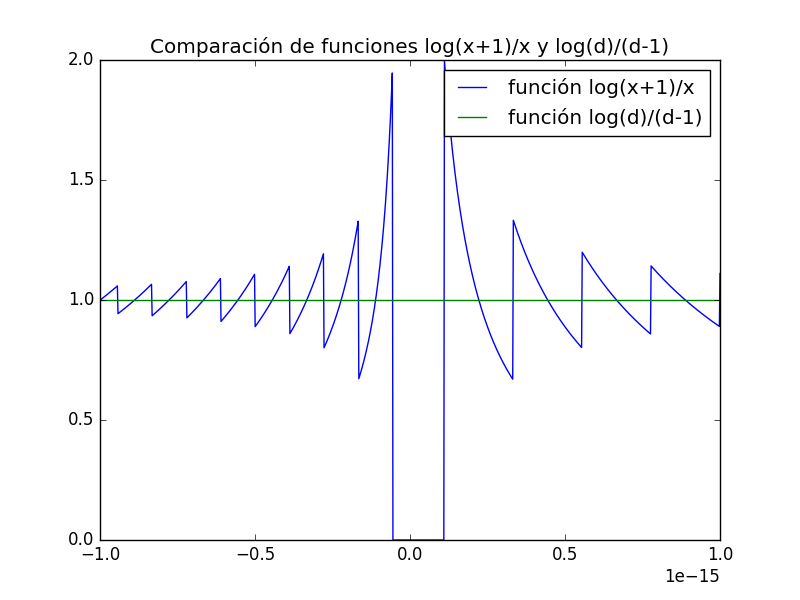
\includegraphics[scale=0.4]{Comparacion_funciones.png}
\caption{Zoom a $x\in [-10^{-15},10^{-15}]$}
\end{minipage}
\end{figure}
\pagebreak
Se muestra el gráfico que compara la misma función solo que con un ajuste ligero que hace una más numéricamente estable. Primero teníamos:
$$f(x) = \frac{\log(x+1)}{x}$$
luego se realiza un cambio de variable y se considera de la siguiente forma.
$$d = x+1 $$
luego 
$$f(d) = \left\lbrace\begin{matrix}
1 &   d = 1\\
\\
\frac{\log(d)}{d-1}&d\neq 1
\end{matrix}\right.$$
De esta forma se logra que la función pierda cifras significativas que alteraban la forma cuando se estaba cerca de cero, y se agrega el límite que falta al indeterminarse la función.\\

En el caso anterior pasaba que como la aritmética no es exacta, se aproximaba el numerador y denominador a su flotante más cercano, lo que generaba diferencias entre ellos, generando así que oscilara la función, al quitarle esas cifras la función es más estable y con la restricción de que $f(d) = 1$ si $d =1$ evita que cuando $x$ sea un número menor al número de máquina este genere errores en el cálculo.
\section*{Pregunta 18}
El producto matricial es equivalente a obtener el producto interno entre la fila de una matriz por la columna de la otra y así obtener el valor correspondiente a cada entrada de la matriz.\\
Como vimos en clases el producto interno podía escribirse como 
$$fl(x^{T}*y)= x^{T}(y+\Delta y)$$
Entonces para cada componente de la matriz $AB$ tendremos algo de esa forma 
por lo que podemos escribirla como:
$$ fl(AB) = (A + \Delta A) B$$
$$ fl (AB) = AB + \Delta AB$$
$$fl(AB)-AB=\Delta AB$$
$$Cond(fl(AB)-AB) \leq Cond(\Delta A)*Cond(B)$$
$$Cond(\Delta A) \leq |\gamma_n|*|A|$$
$$Cond(B)= |B|*|B^{-1}|$$
Entonces nos queda la siguiente igualdad:
$$Cond(fl(AB)-AB)\leq |\gamma_n|*|A|*|B|*|B^{-1}|  $$
El backward error será pequeño si es que la matrices $A$ y $B$ están bien condicionadas.
\section*{Pregunta 27}
Sean $A$ y $C$ matrices cuadradas, y se tiene la matriz ortogonal particionada:
$$\left\rbrace
\begin{bmatrix}
A&B\\
0&C
\end{bmatrix}\right.
$$
Se pide probar que $A$ y $C$ son ortogonales y que $B$ es la matriz nula.\\

Para eso, como es una matriz ortogonal debe cumplir que:
$$
\begin{bmatrix}
A & B\\
0 & C
\end{bmatrix}
*
\begin{bmatrix}
A^{T}& 0\\
B^{T} & C^{T}
\end{bmatrix}
=
\begin{bmatrix}
A*A^{T} + B*B^{T}& B*C^{T}\\
C*B^{T}& C*C^{T}
\end{bmatrix}
=
I$$
Luego notamos que se debe cumplir las siguientes ecuaciones
\begin{equation}
C*C^{T}=I
\end{equation}
Entonces $C$ es ortogonal
\begin{equation}
C*B^{T}=0
\end{equation}
\begin{equation}
B*C^{T}=0
\end{equation}
Para ambos casos se debe cumplir que $B$ es cero ya que al ser $C$ ortogonal, es de rango completo entonces su kernel es solamente el vector cero, por lo que $B$ y $B^{T}$ deben ser la matriz nula.
\begin{equation}
A*A^{T}+B*B^{T}=I
\end{equation}
por lo anterior se cumple 
$$A*A^{T} + \cancel{B*B^{T}}=I$$
$$A*A^{T} = I$$
Entonces $A$ es ortogonal.
\end{document}